\documentclass[a4paper]{article}

\usepackage[utf8]{inputenc}
\usepackage[T1]{fontenc}
\usepackage{textcomp}
\usepackage[english]{babel}
\usepackage{amsmath, amssymb}


%figure support
\usepackage{import}
\usepackage{xifthen}
\pdfminorversion=7
\usepackage{pdfpages}
\usepackage{transparent}
\newcommand{\incfig}[1]{%
	\def\svgwidth{\columnwidth}
	\import{./figures/}{#1.pdf_tex}
}
\graphicspath{ {./figures/} }
\pdfsuppresswarningpagegroup=1

\begin{document}
	\title{EEL4768C.04 Homework 5 Due 11/19/19}
	\author{Brandon Thompson 5517}
	\maketitle

	\begin{enumerate}
		\item Modify the multi-cycle MIPS processor to implement the \verb|jr| instruction.
			See Appendix B for instruction definitions. Mark up a copy of figure
			\ref{fig:c_multicycle_processor} to indicate changes to the datapath. Name any new
			control signals. Mark up a copy of figure \ref{fig:c_multicycle_fsm} to show changes
			to the controller FSM. Describe any other changes that are required.\\
			\\
			\texttt{jr} updates PC with the value in the specified register.\\
			\verb|jr| functionality has already been implemented in figure \ref{fig:c_multicycle_processor}, no changes necessary.
			\begin{figure}[ht!]
				\centering
				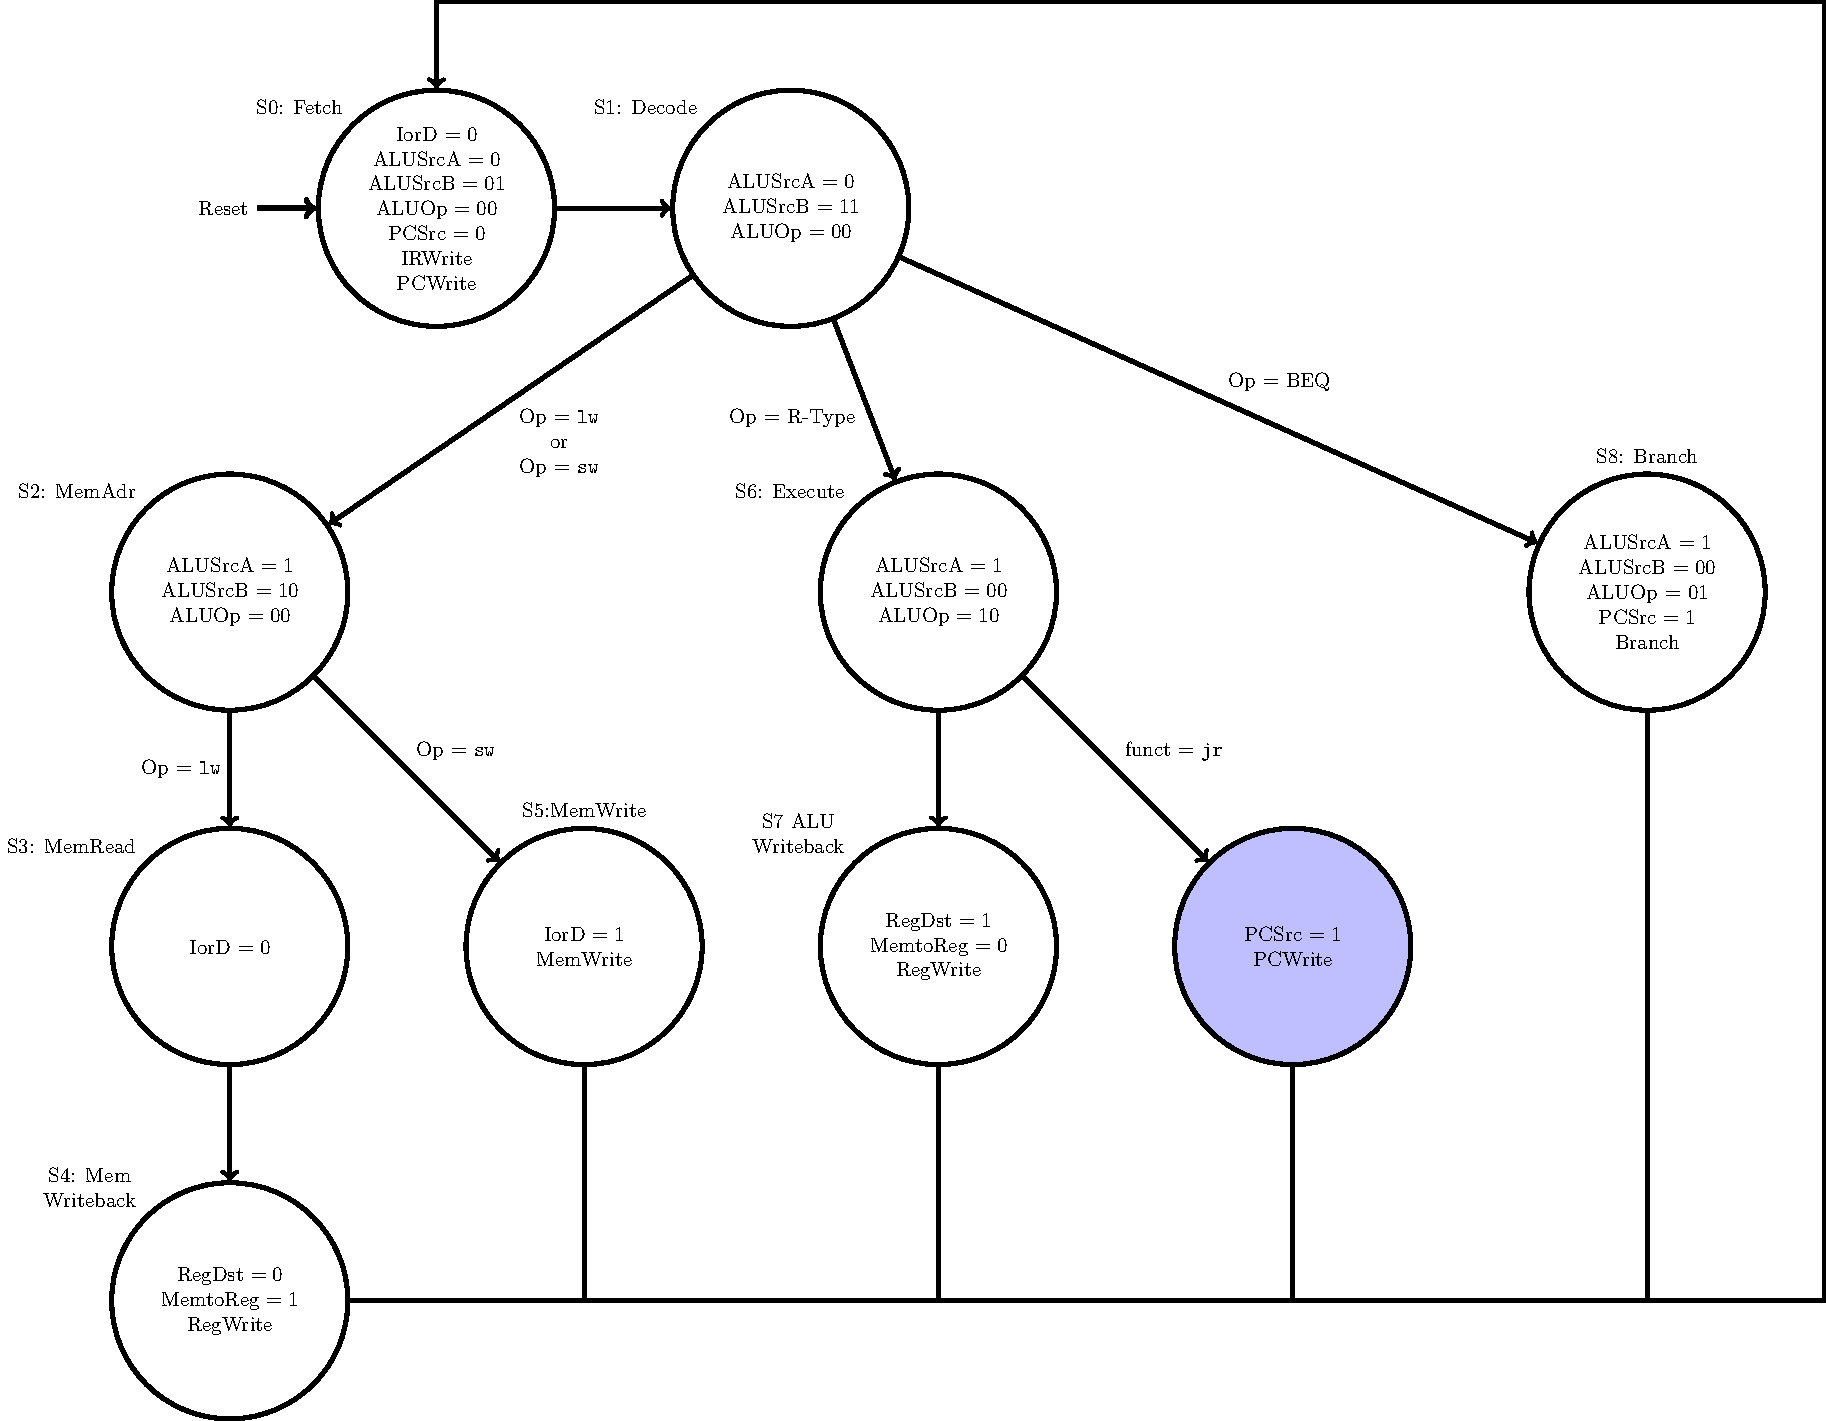
\includegraphics[width=\textwidth]{ca_hw5_q1b}
				\caption{MIPS FSM including \texttt{jr} instruction.}
				\label{fig:ca_hw5_q1b}
			\end{figure}
			
			\clearpage
		\item Repeat for the \verb|bne| instruction.\\
			\\
			\texttt{bne} checks if two registers are not equal. If they are not equal,
			go to branch target address. Else, go to next instruction.
			\begin{figure}[ht]
				\centering
				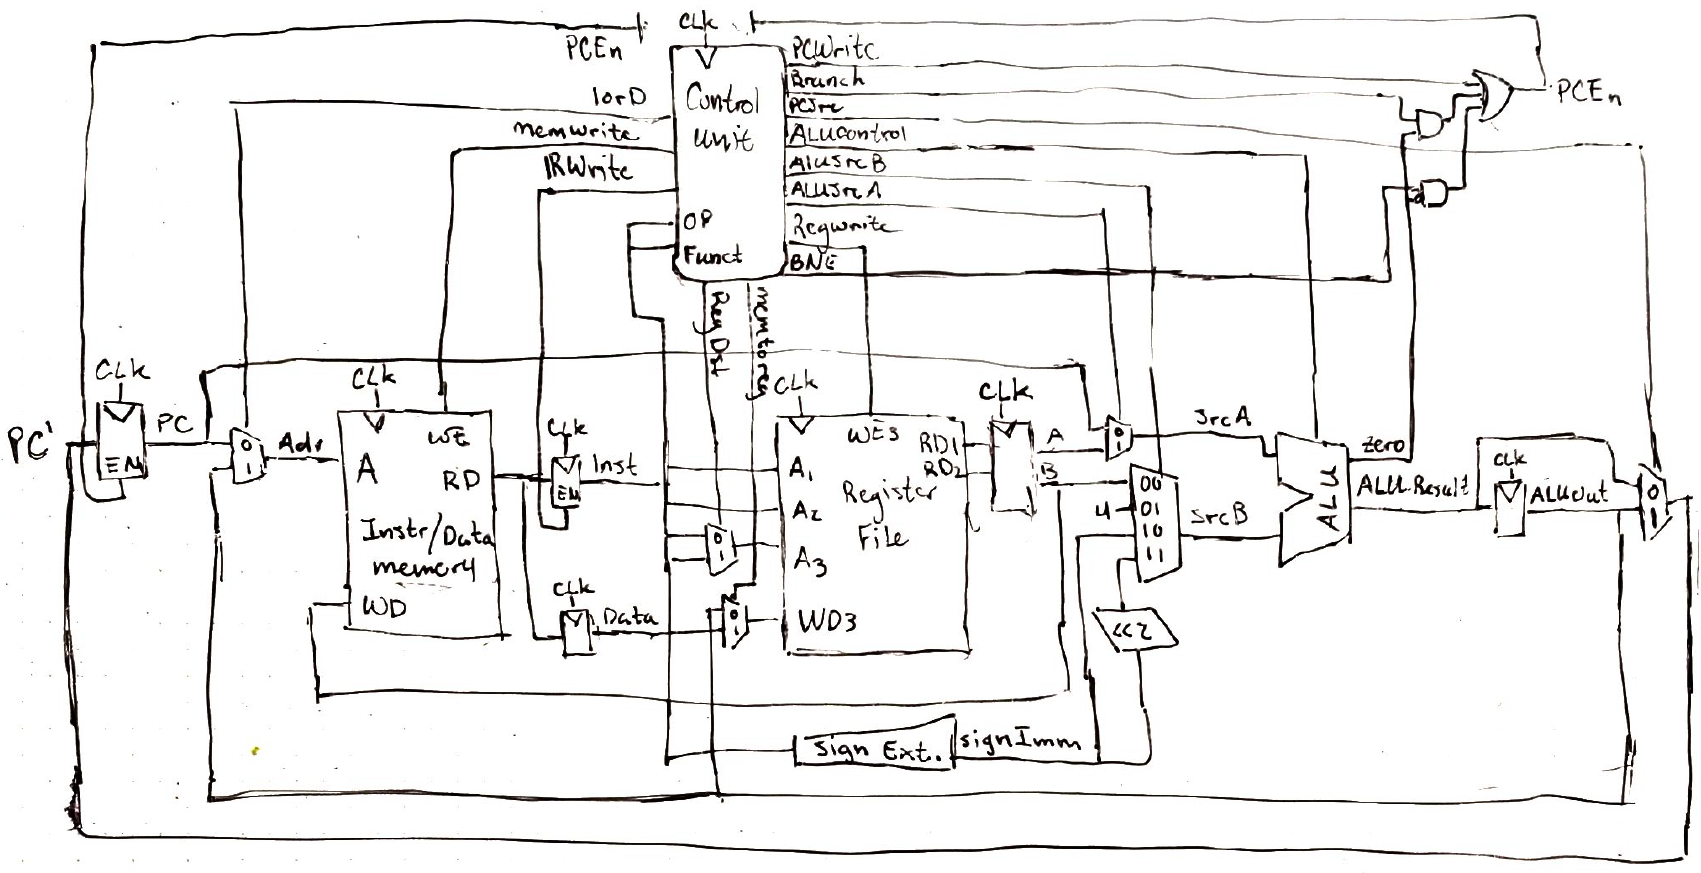
\includegraphics[width=\textwidth]{ca_hw5_q2a}
				\caption{MIPS multi-cycle processor with \texttt{bne} implemented.}
				\label{fig:ca_hw5_q2a}
			\end{figure}
			\begin{figure}[ht]
				\centering
				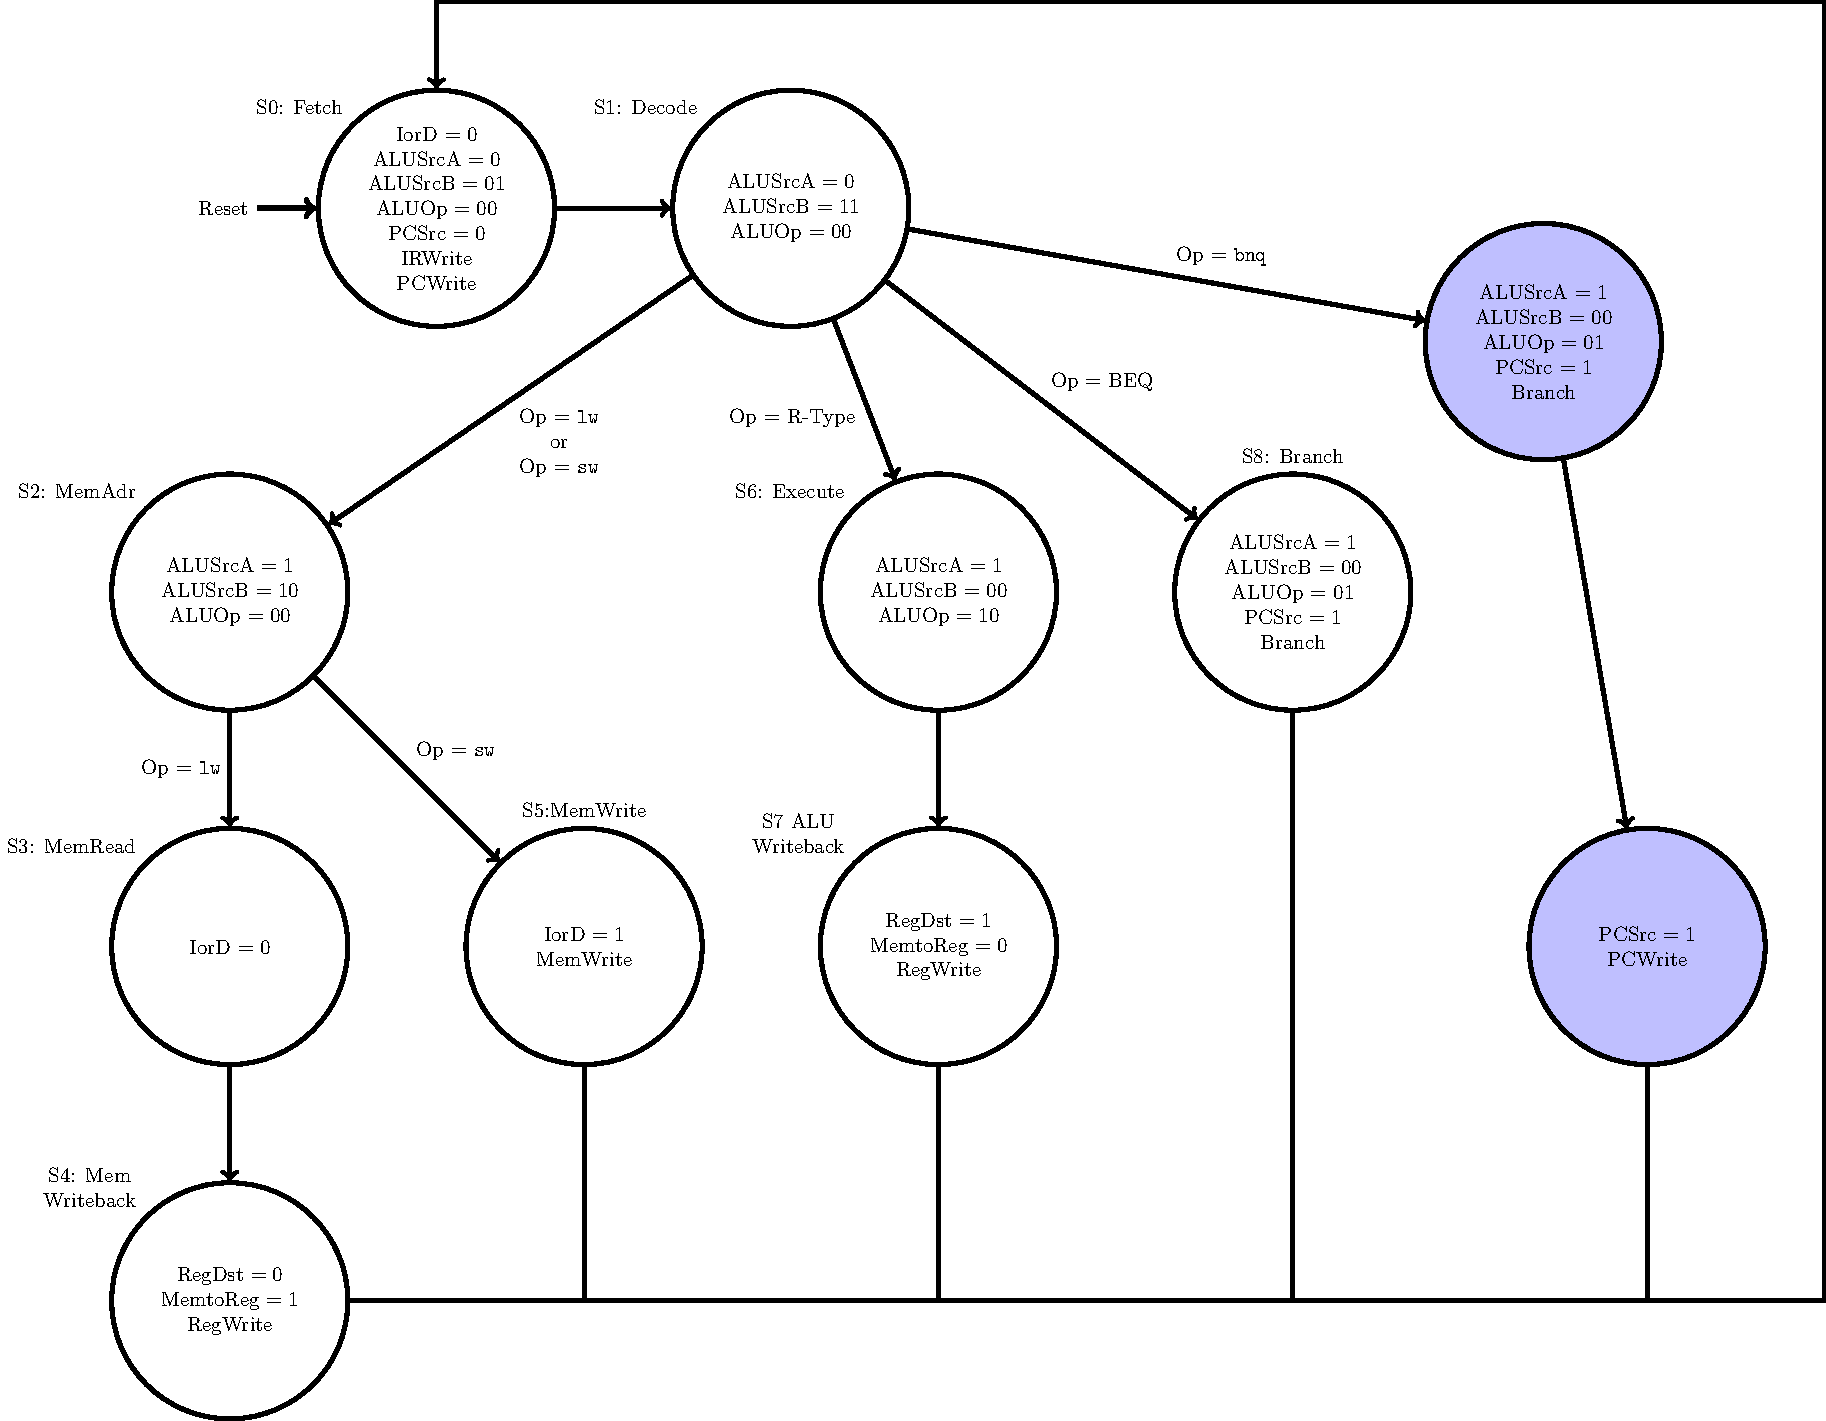
\includegraphics[width=0.8\textwidth]{ca_hw5_q2b}
				\caption{MIPS FSM including \texttt{bne} instruction.}
				\label{fig:ca_hw5_q2b}
			\end{figure}
	\end{enumerate}
\clearpage
	\begin{figure}[ht!]
		\centering
		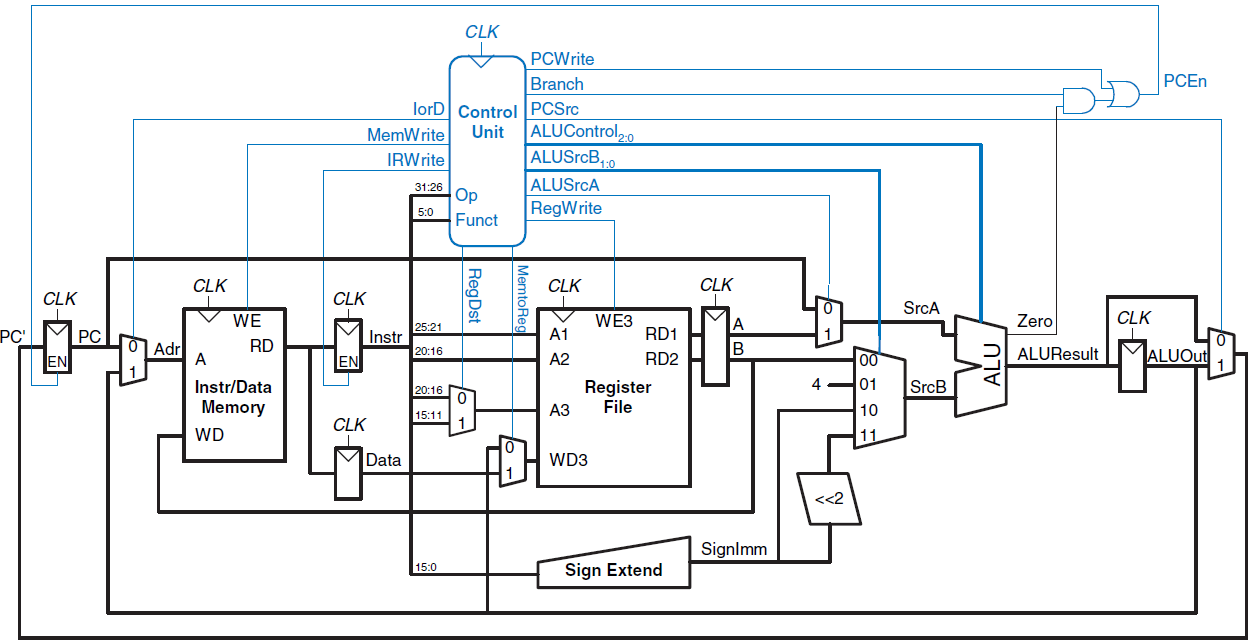
\includegraphics[width=0.8\textwidth]{7_27}
		\caption{Complete multicycle MIPS processor \textbf{(EDIT THIS)} .}
		\label{fig:c_multicycle_processor}
	\end{figure}
	\begin{figure}[ht!]
		\centering
		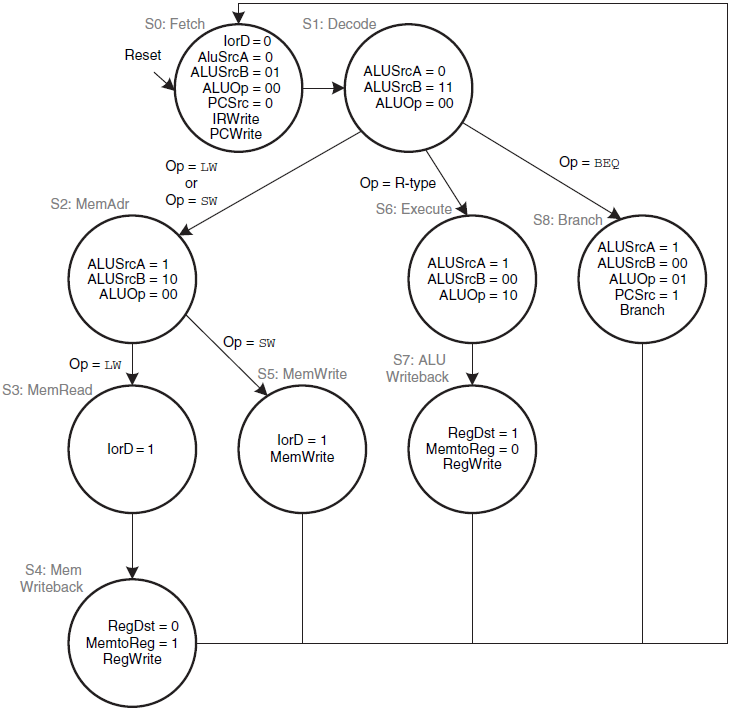
\includegraphics[width=0.8\textwidth]{7_39}
		\caption{Complete multicycle control FSM \textbf{(EDIT THIS)}.}
		\label{fig:c_multicycle_fsm}
	\end{figure}
\end{document}
